%!TEX root = ../main.tex

\newpage
\section*{Supplementary figures}

  \renewcommand{\thefigure}{S\arabic{figure}}
  \setcounter{figure}{0}

  \begin{figure}[h]
  \centering
  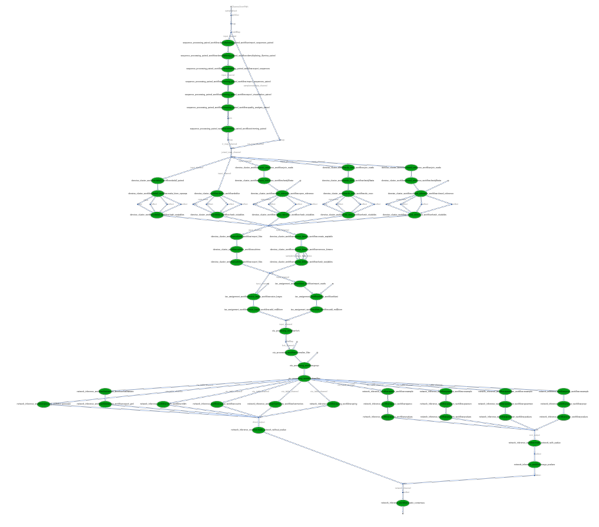
\includegraphics[width=0.67\linewidth]{figureS1.pdf}
  \caption{
    \textbf{Comparison of various denoising and clustering algorithms used in the pipeline}.
    (A, B) Correlation of the abundances of the taxa that are common between the count matrices created by two different methods.
    (A) The best correlation (most similar methods) is between open-reference and denovo.
    (B) The worst correlation (least similar methods) is between open-reference and dada2.
    (C) A heatmap showing the $\mathrm{R}^2$ of all pairwise comparisons of the methods.
  }
  \label{fig:figureS1}
\end{figure}

  \begin{figure}[h]
    \centering
    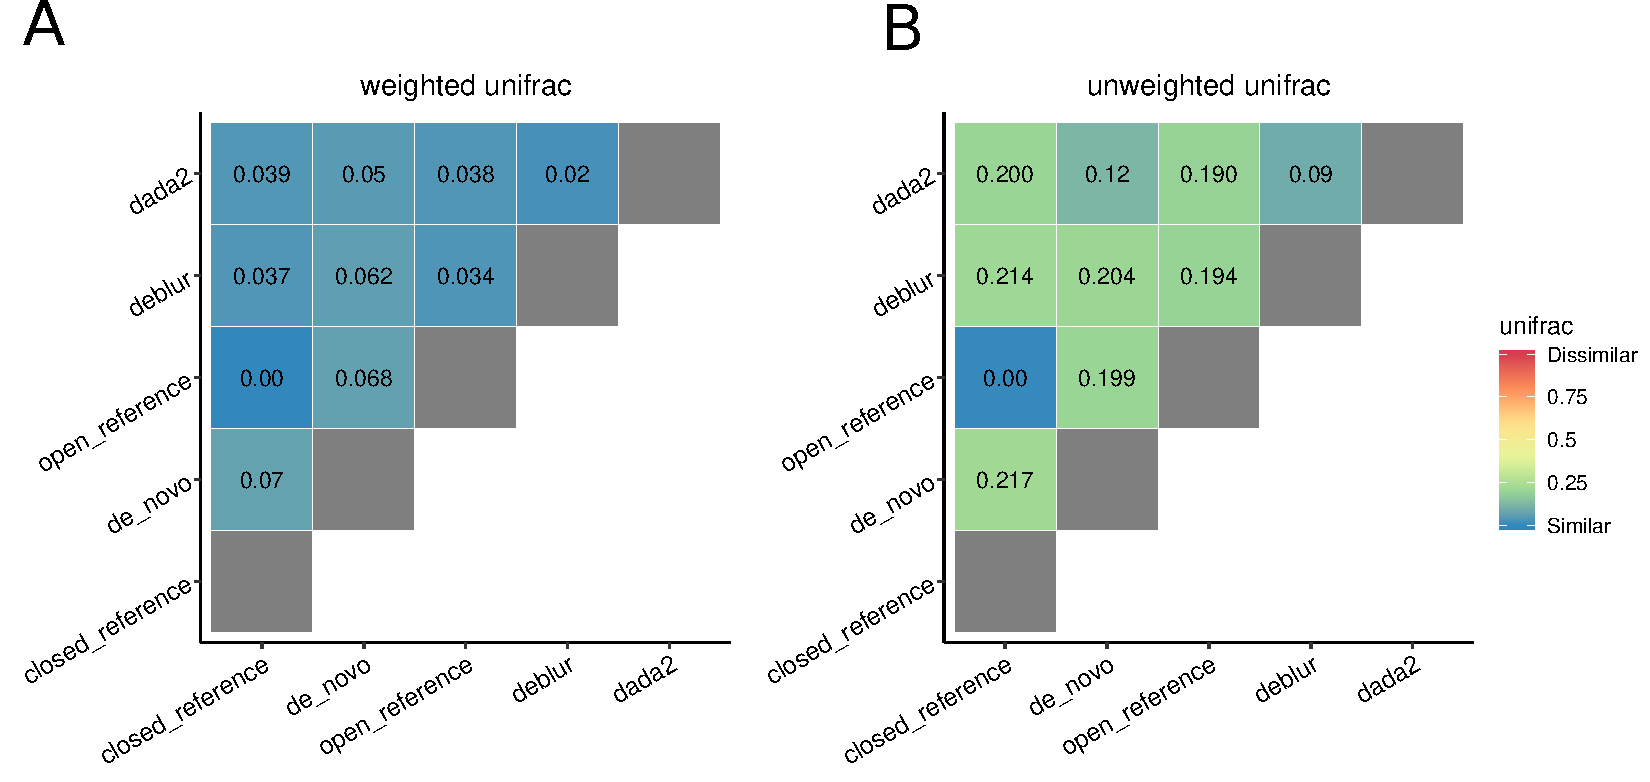
\includegraphics[width=0.8\linewidth]{figureS2.pdf}
    \caption{Results of the mock community analysis. (A) Weighted unifrac (B) Unweighted unifrac}
    \label{fig:figureS2}
  \end{figure}

  \begin{figure}[h]
    \centering
    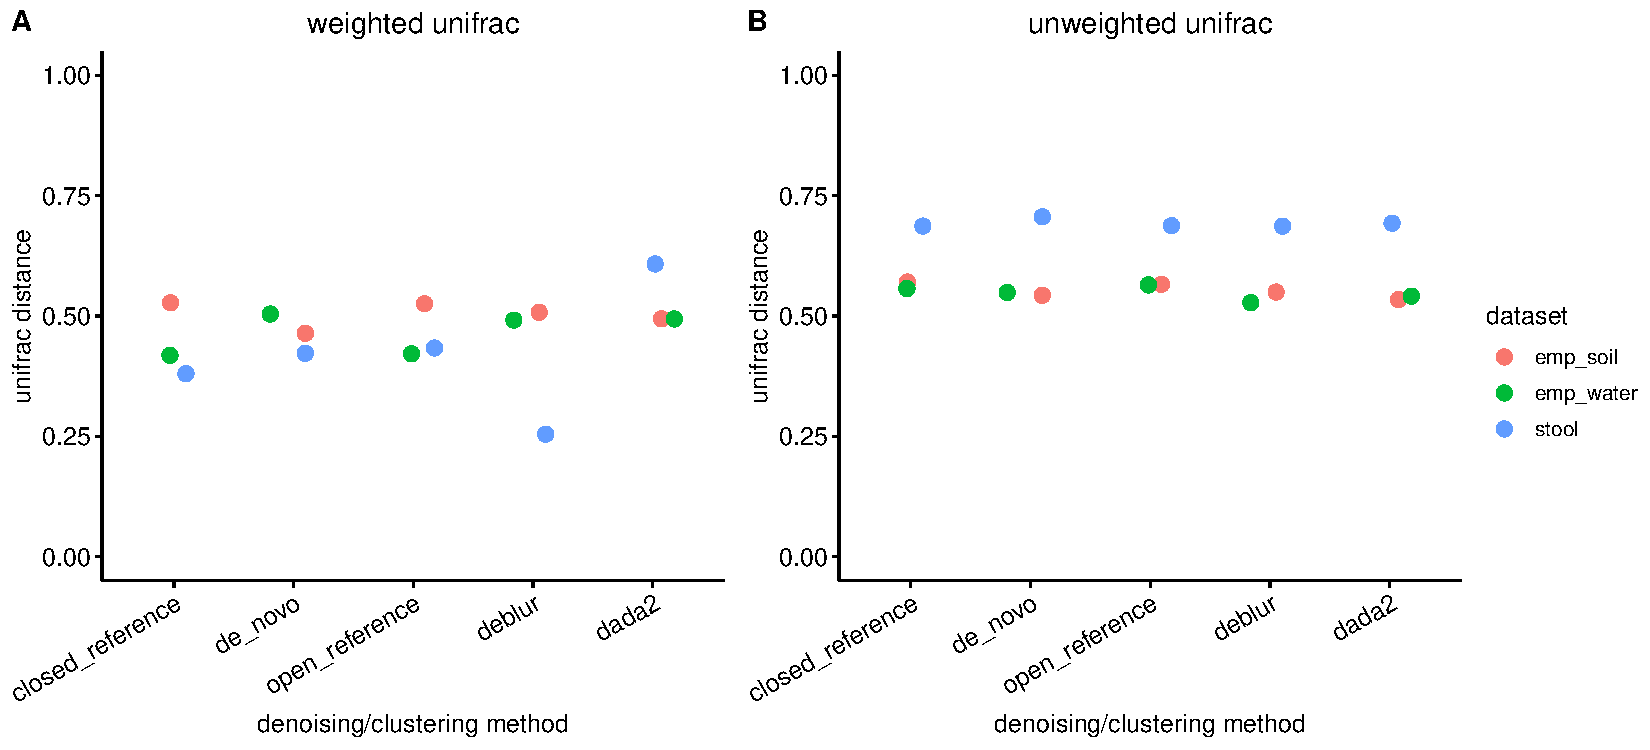
\includegraphics[width=0.8\linewidth]{figureS3.pdf}
    \caption{Results of the synthetic community analysis. (A) Weighted unifrac (B) Unweighted unifrac}
    \label{fig:figureS3}
  \end{figure}

  \begin{figure}[h]
    \centering
    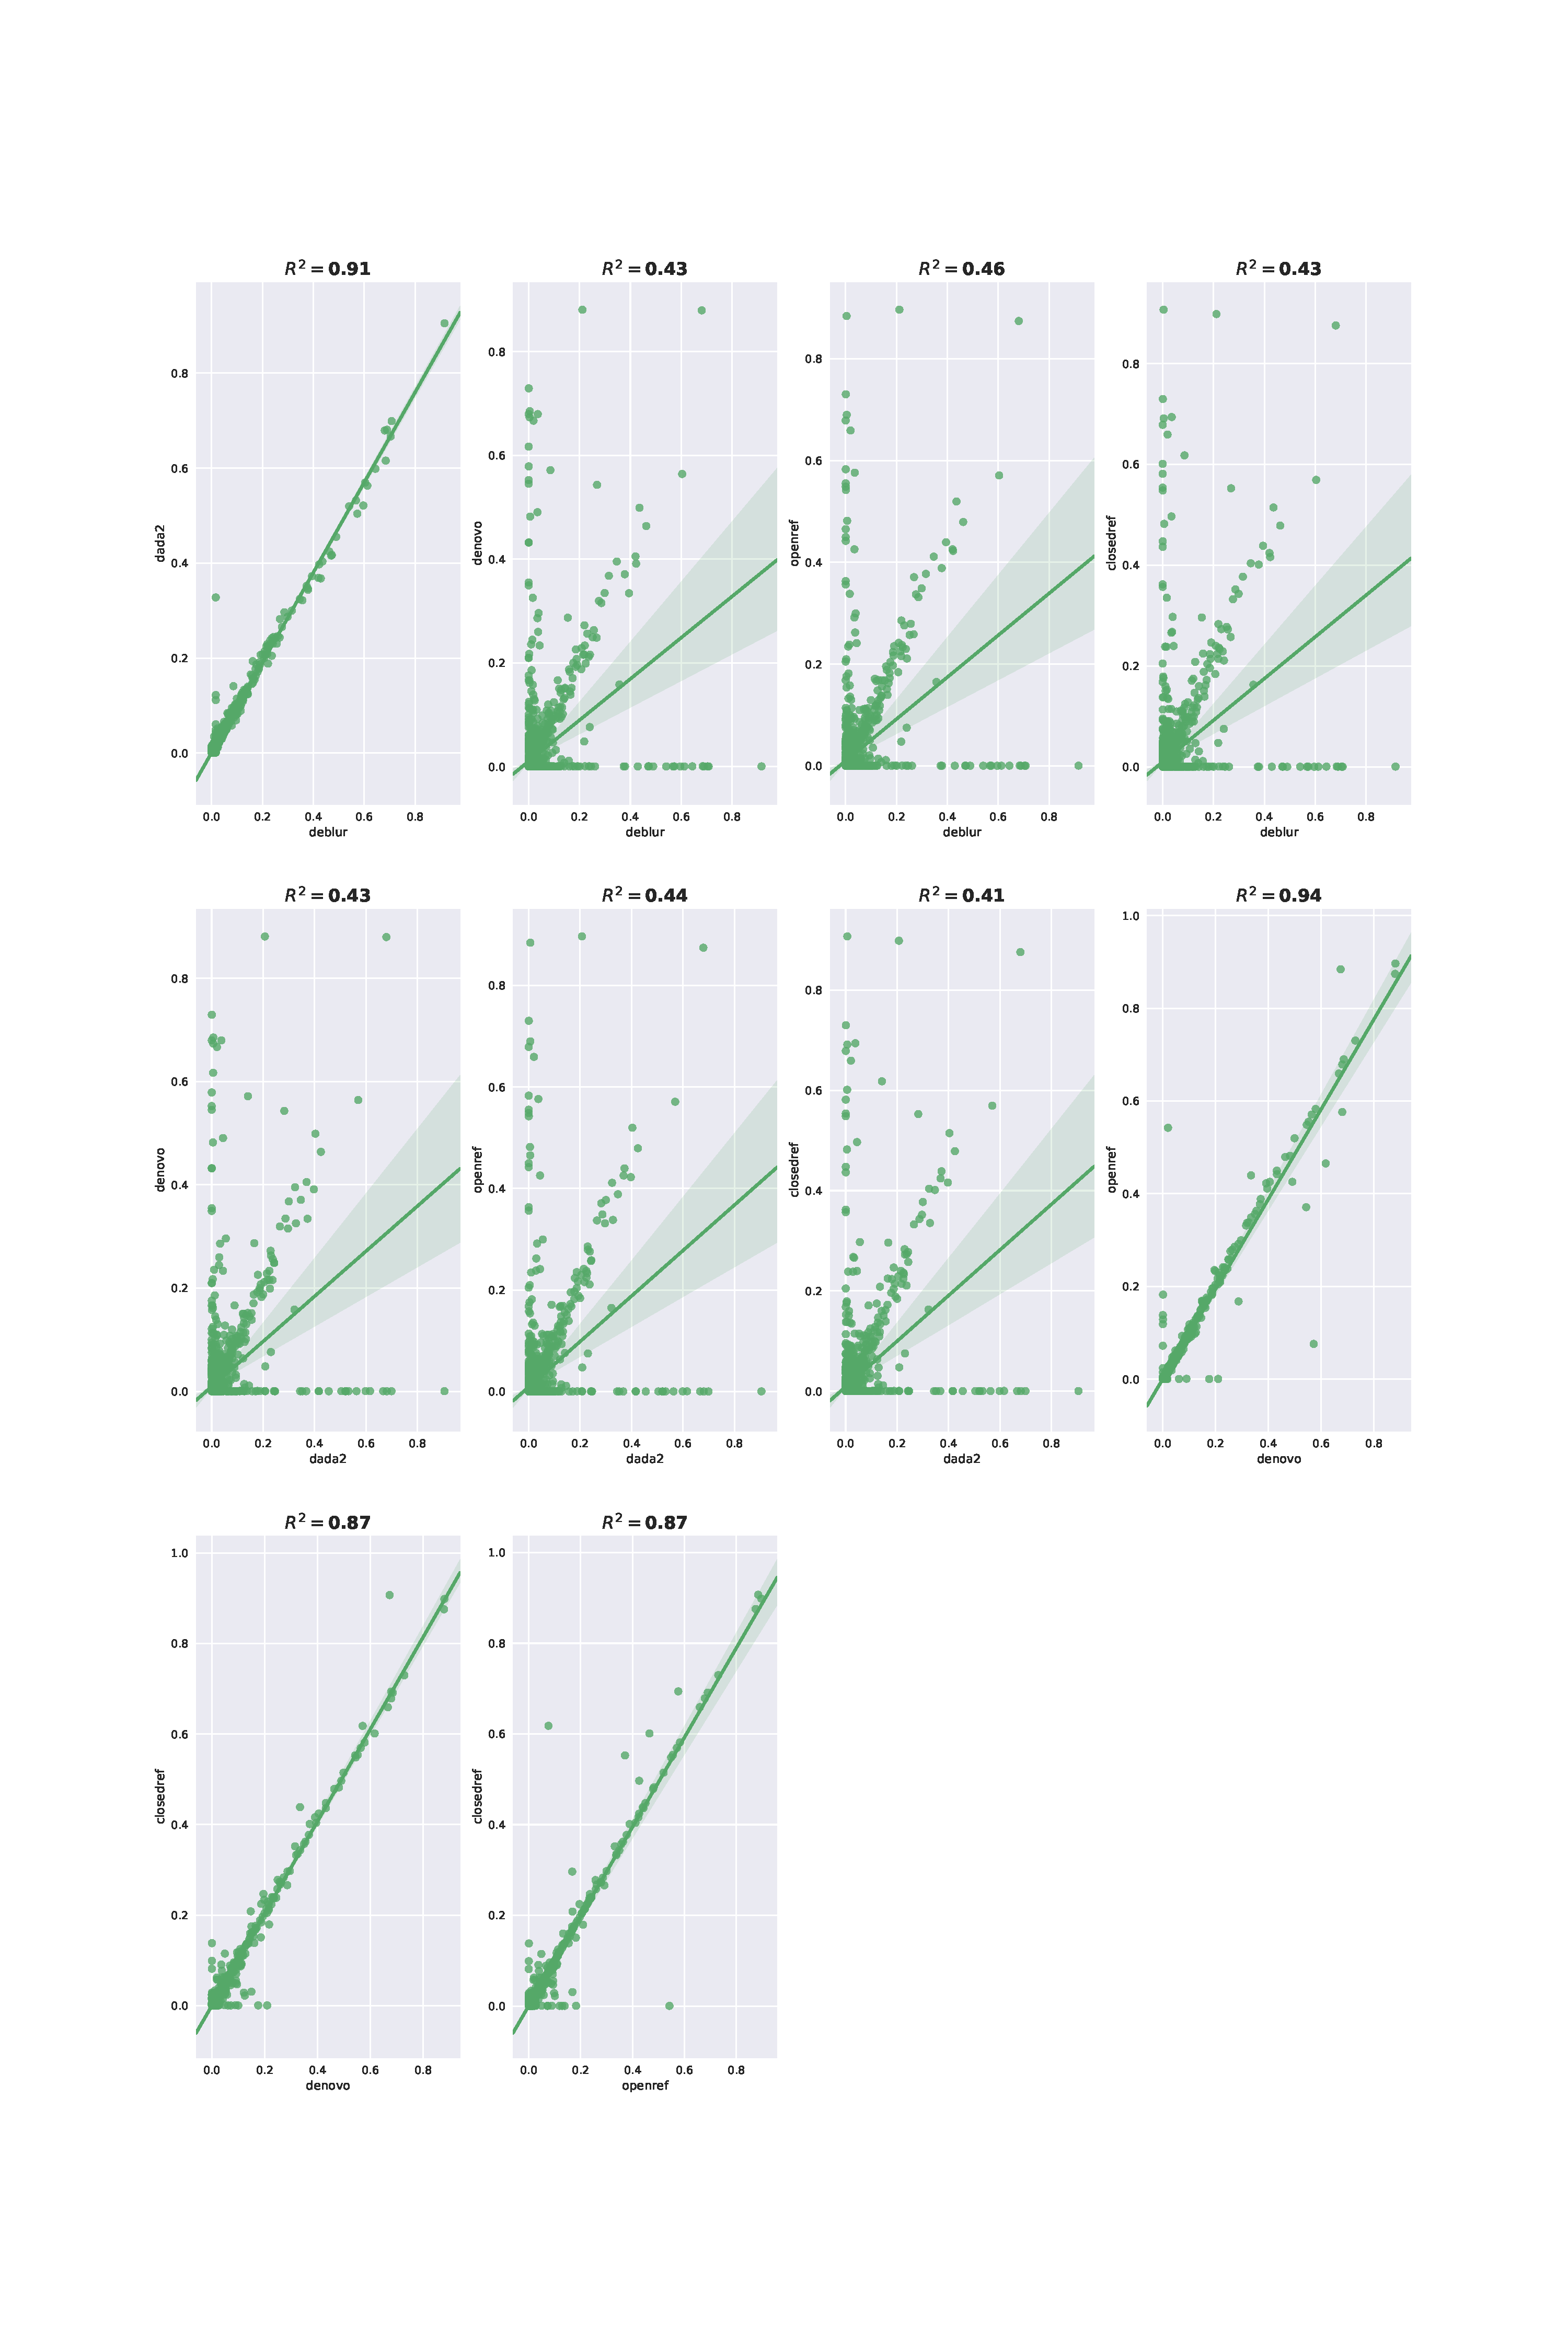
\includegraphics[width=0.8\linewidth]{pdf/all_denoise_reg.pdf}
    \caption{All pairwise correlations comparing the similarity between different denoising and clustering methods}
    \label{fig:figureS4}
  \end{figure}

  \begin{figure}[h]
    \centering
    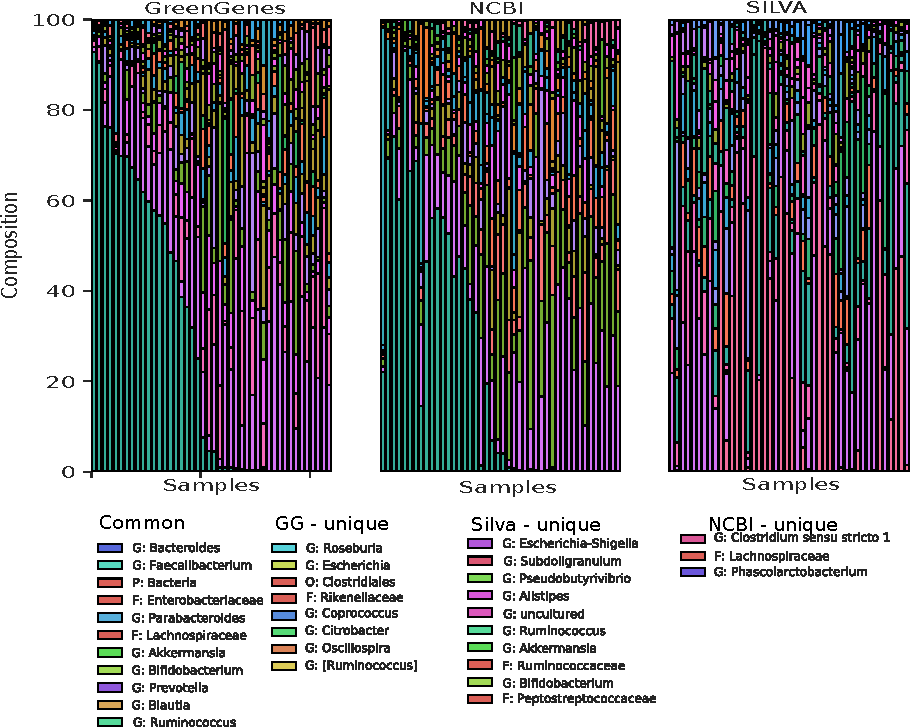
\includegraphics[width=\linewidth]{figureS4.pdf}
    \caption{
      \textbf{(A)} Taxonomy composition of the 20 most abundant genera predicted using different taxonomy references databases: Greengenes, SILVA and NCBI.
      The legend shows the common and the unique genera among the taxonomy assignments.
  }
    \label{fig:figureS4}
  \end{figure}

  \begin{figure}[h]
    \centering
    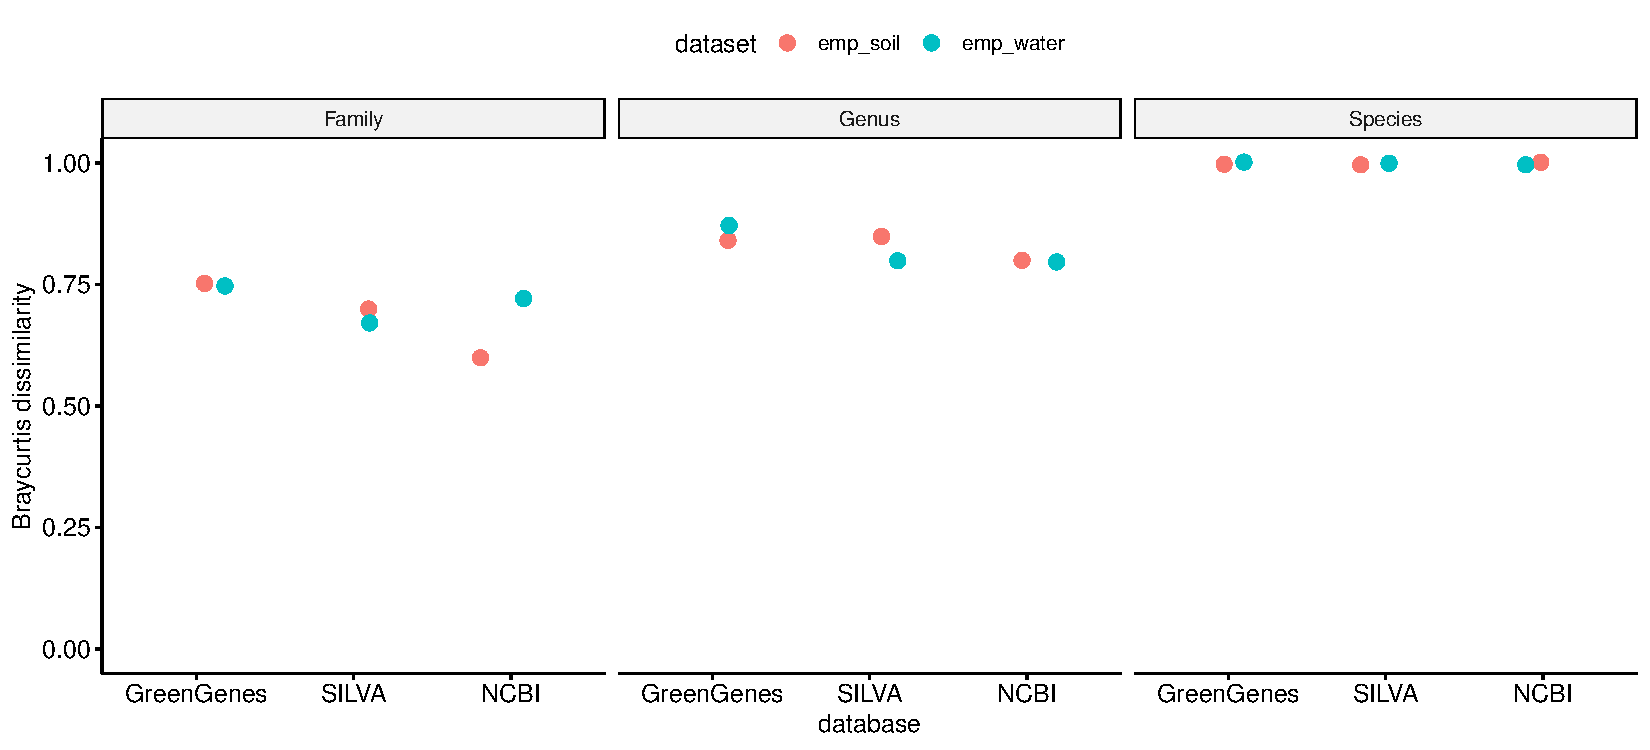
\includegraphics[width=\linewidth]{figureS5.pdf}
    \caption{
      The bray-curtis dissmilarity between the expected taxonomic composition and generated taxonomic composiion for the synthetic datasets.
  }
    \label{fig:figureS4}
  \end{figure}

  \begin{figure}[h]
    \centering
    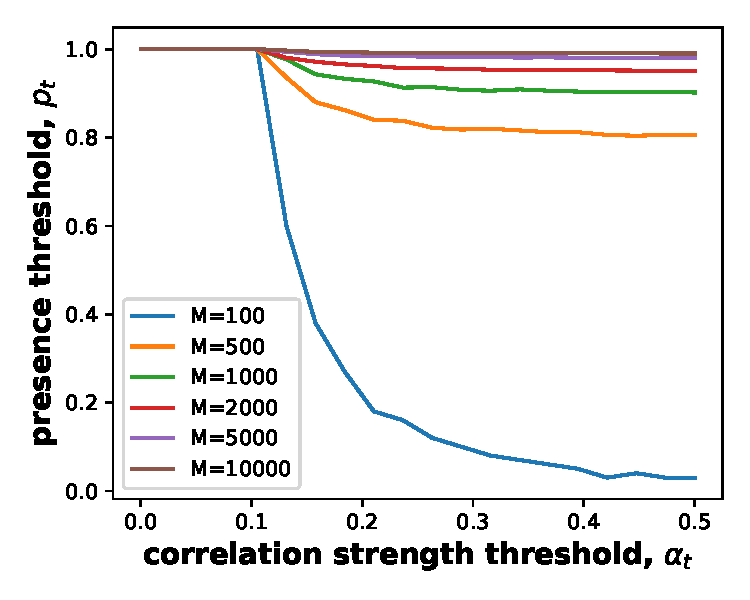
\includegraphics[width=\linewidth]{figureS6.pdf}
    \caption{
      The effect of OTU processing measurs on the OTU table
  }
    \label{fig:figureS4}
  \end{figure}

  \begin{figure}[h]
    \centering
    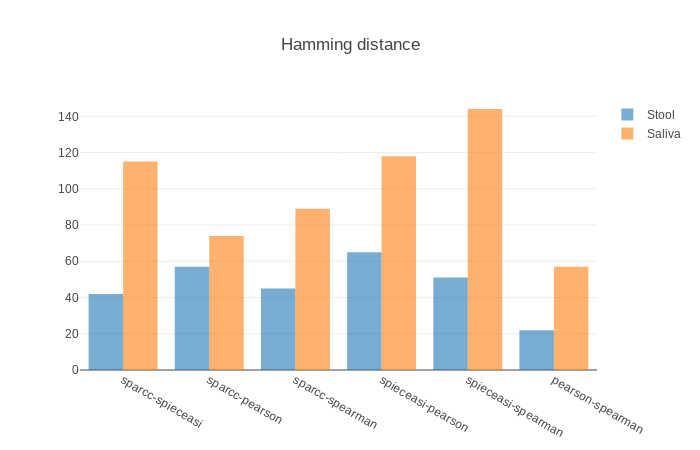
\includegraphics[width=0.8\linewidth]{png/hamming_distance.png}
    \caption{The hamming distance between the networks is shown. The similarity between various methods was found to vary with the data-source used.}
    \label{fig:figureS4}
  \end{figure}

  \begin{figure}[h]
    \centering
    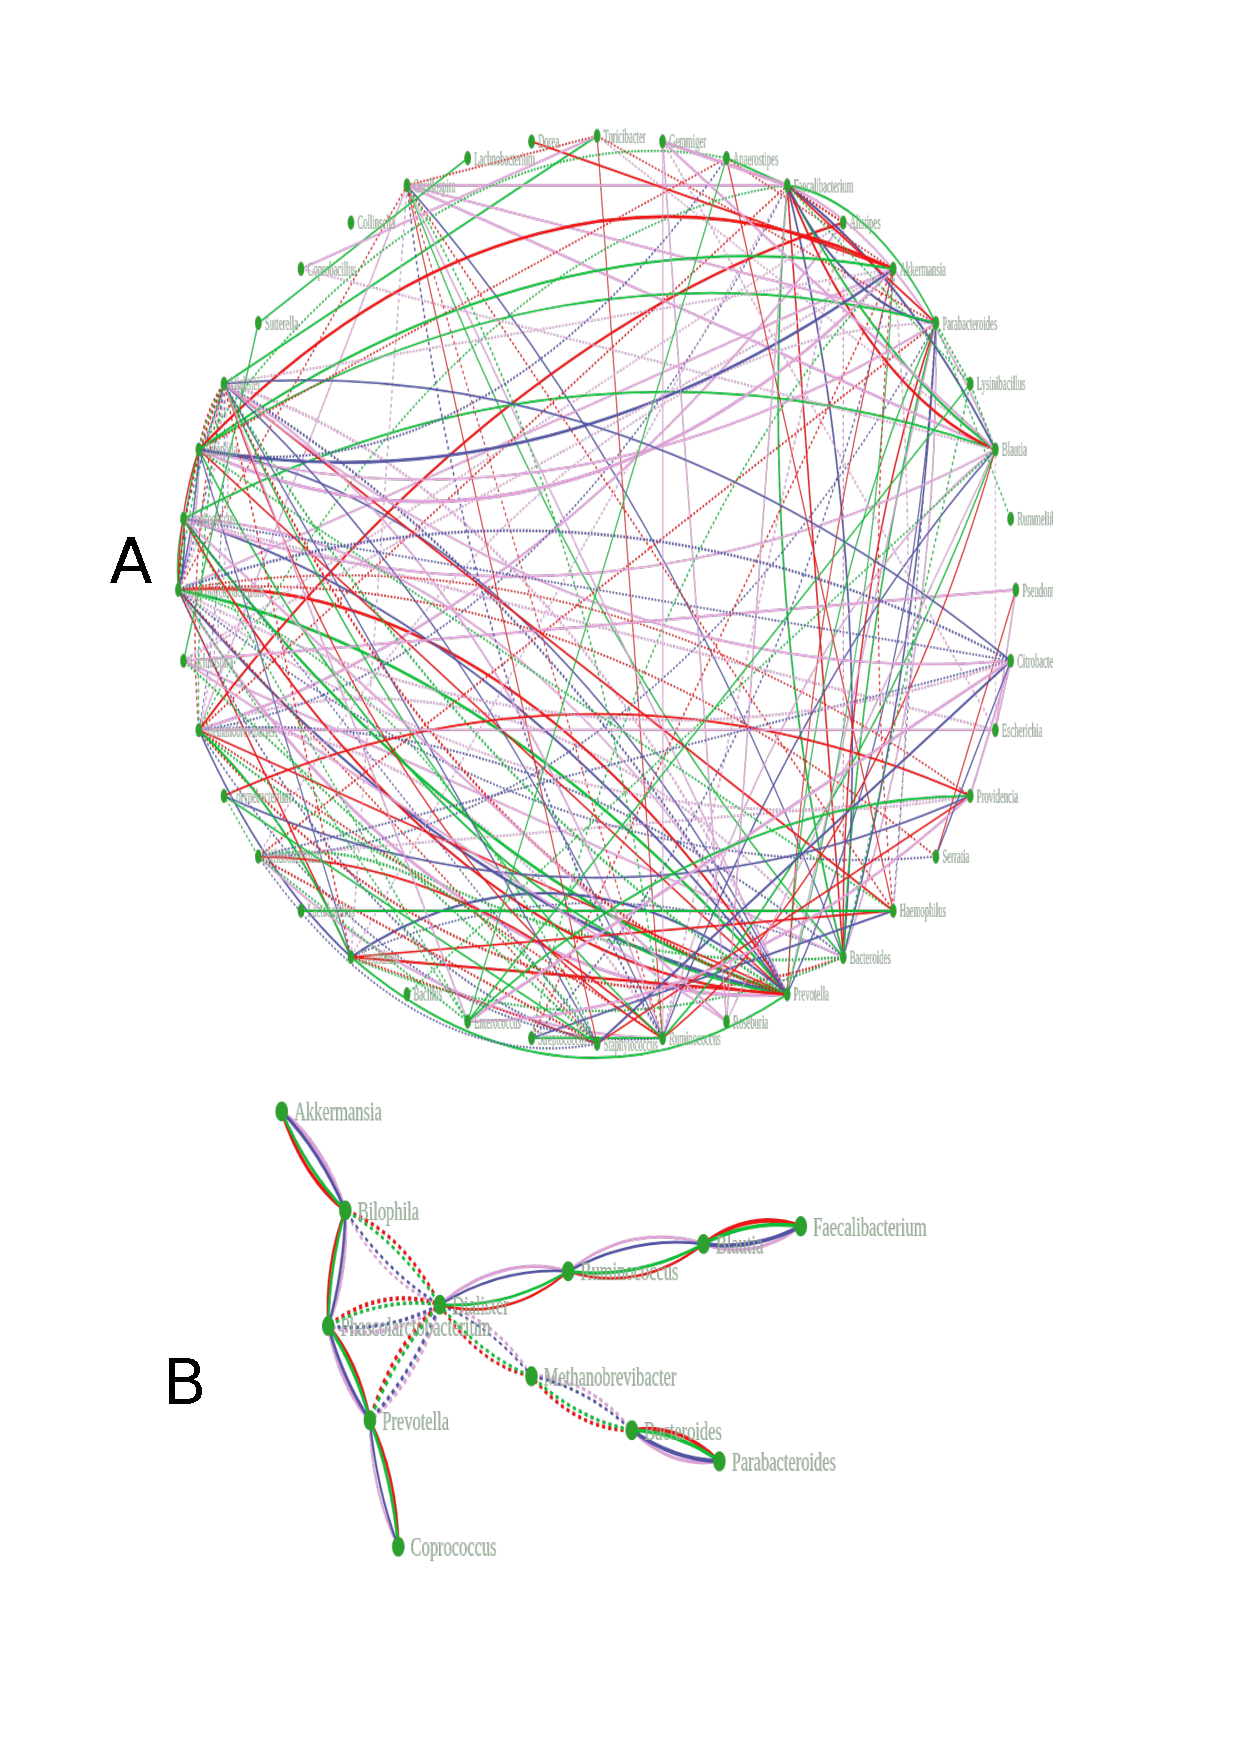
\includegraphics[width=0.8\linewidth]{pdf/denoise_network.pdf}
    \caption{A network showing union and intersection of networks generated using certain combination of methods}
    \label{fig:figureS5}
  \end{figure}
